\section{A finite certificate at the coloring boundary}
\label{grid:section}

We now prove non-reconstruction at the remaining negative equalities, including
the channel $\lambda=-1/2$.  Throughout this section $a=-\lambda>0$,
$p=(p_0,p_1,p_2)$ is a posterior probability vector, and
$\zeta=\sum_{i=0}^2p_i\omega^i$, where $\omega=e^{2\pi\mathrm{i}/3}$.
In this section the input spin $S$ denotes its index in $\{0,1,2\}$;
its complex representative is $\omega^S$.
Write $\mu=\E|\zeta|^2$.  Proposition~\ref{loc:gap} says that a symmetric
fixed point at $da^2=1$ with $\mu\leq 1/20$ is the uniform posterior.
It will therefore suffice to dominate one finite-depth experiment by an
explicit experiment with $\mu<1/20$.  The dominating process need not itself
be at equality or converge to the uniform posterior.

\subsection{Explicit refinements of posterior experiments}

The finite representation follows the survey method of Bhatnagar and
Maneva~\cite[Sections~3.1--3.3 and Theorems~5--8]{BhatnagarManeva2011}:
posterior vectors are replaced by barycentric mixtures on a finite grid,
and rounding deficits and omitted offspring tails are completed by
perfectly informative messages. We give explicit refinement kernels for
every operation and exact arithmetic certificates for the three-state
parameter ranges used here.

For experiments with the same input spin $S$, write $\mathcal E\preceq
\mathcal F$ if a Markov kernel, independent of $S$, transforms the data of
$\mathcal F$ into data with the conditional laws of $\mathcal E$.
Such a kernel is called a garbling.  Under the uniform prior, an experiment
with datum $Y$, marginal law $\rho$, and posterior $p(Y)$ satisfies
\begin{equation}
 \PP(S=i,Y\in dy)=p_i(y)\rho(dy),\qquad
 \PP(Y\in dy\mid S=i)=3p_i(y)\rho(dy).
 \label{grid:canonical}
\end{equation}
Its full labeled posterior is an equivalent experiment: the reverse kernel
from $p$ to $Y$ is the conditional marginal law $\rho(dy\mid p(Y)=p)$.
Equation~\eqref{grid:canonical} proves that this kernel also works under
every input spin.  All conditional distributions used here exist on the
finite or standard Borel spaces in question.

We compress a permutation-invariant posterior law by storing one mass for
each orbit under the six coordinate permutations.  The represented datum
is always the \emph{full labeled posterior}. Under its marginal law, draw
an orbit, uniformly permute its representative, and retain the resulting
vector. Repeated
coordinates cause no difficulty, since each distinct orientation has the
same multiplicity among the six permutations.  Observing only the orbit
index would be a different experiment and is not used below.

\begin{lemma}[Barycentric refinement]
\label{grid:spread}
Suppose that for every old datum $y$ there are probabilities
$\alpha_y(z)$ on a finite set of posterior vectors such that
$\sum_z\alpha_y(z)z=p(y)$.  Then the posterior law
$\nu(z)=\int\alpha_y(z)\rho(dy)$ defines an experiment that dominates the
old one.
\end{lemma}
\begin{proof}
Here is an explicit refinement conditional on the input spin.  Given
$S=i$ and $Y=y$ with $p_i(y)>0$, choose $z$ with probability
\begin{equation}
 R_i(y,z)=\frac{\alpha_y(z)z_i}{p_i(y)}.
 \label{grid:spread-forward}
\end{equation}
Choose any distribution on the null event $p_i(y)=0$.  The barycenter
identity makes this a probability kernel.  Its joint law is
$\PP(S=i,Y\in dy,Z=z)=\rho(dy)\alpha_y(z)z_i$, so that the posterior
given $(Y,Z)$ is $Z$.  After retaining just $Z$, the reverse garbling is
\begin{equation}
 G(z,dy)=\frac{\rho(dy)\alpha_y(z)}{\nu(z)}\quad\text{if }\nu(z)>0.
 \label{grid:spread-reverse}
\end{equation}
It is independent of $i$ and recovers the old conditional law, since
$\sum_z3z_i\nu(z)G(z,dy)=3p_i(y)\rho(dy)$.  Arbitrary kernels at
$\nu(z)=0$ are harmless.  In particular $\alpha_y$ specifies
\emph{marginal} spreading probabilities; the actual refinement conditional
on the spin is~\eqref{grid:spread-forward}.
\end{proof}

\begin{lemma}[Symmetric completion by pure posteriors]
\label{grid:completion}
Let a finite symmetric posterior law have orbit masses $W_o$, and suppose
$0\leq L_o\leq W_o$ for each orbit.  The law retaining masses $L_o$ and
putting the remaining mass $1-\sum_oL_o$ at the uniformly permuted pure
orbit dominates the original experiment.
\end{lemma}
\begin{proof}
On a datum $p$ in orbit $o$, retain $p$ with probability
$t(p)=L_o/W_o$ (put $t=0$ when $W_o=0$).  Otherwise reveal the input spin.
More precisely, conditional on $(S=i,p)$ the refined datum is $(p,0)$
with probability $t(p)$ and $(p,1,i)$ otherwise.  Forgetting the flag and
the revealed spin recovers $p$, so this is a refinement.  The respective
posteriors are $p$ and $e_i$, and their full posterior is sufficient by
\eqref{grid:canonical}.  Removal is constant across each orbit, whence
\[
 \PP(S=i,\text{removed from }o)
   =(W_o-L_o)\frac16\sum_{\pi\in\mathfrak S_3}(\pi p)_i
   =\frac{W_o-L_o}{3}.
\]
Thus the revealed part is exactly the stated pure orbit, with no change
to the uniform input prior. This also covers removal from the pure orbit:
retaining a pure posterior and revealing the already known spin are
disjoint flagged outcomes that compress to the same posterior, so their
masses add.
For completeness, if $\rho(p)$ denotes an old labeled posterior mass and
$\nu(z)$ the resulting mass, the reverse kernel after posterior
compression is explicitly
\[
 G(z,p)=\frac{\rho(p)}{\nu(z)}
 \left[t(p)\mathbf1_{\{z=p\}}+
 (1-t(p))\sum_{i=0}^2p_i\mathbf1_{\{z=e_i\}}\right]
 \quad(\nu(z)>0).\qedhere
\]
\end{proof}

Both independent composition and edge transmission preserve
$\preceq$.  In detail, if $G_j$ garbles the $j$th upper branch into the
$j$th lower branch, instantiate the upper branch data independently
\emph{conditional on their common input spin}, and use the product
kernel $\prod_jG_j$ with independent auxiliary randomness.  Under each
input this recovers the product of the lower conditional laws.  For an
edge, averaging these same conditional identities against the channel
$K_\lambda(i,j)$ proves the claim.  Mixing over an input-independent
count also preserves the order: retain the count and apply the appropriate
product garbling conditional on it.  These facts justify each induction
below; no monotonicity of the numerical rounding map is assumed.

\subsection{Grid spreading and exact product tables}

Fix
\[
 H=72,\qquad N=10^{12},\qquad
 \mathcal H=\{(h_0,h_1,h_2)\in\mathbb Z_{\geq0}^3:
     h_0\geq h_1\geq h_2,\ h_0+h_1+h_2=H\}.
\]
There are $469$ representatives in $\mathcal H$.  An integer vector of
nonnegative masses $(m_h)_{h\in\mathcal H}$ summing to $N$ represents the
symmetric posterior law with orbit probabilities $m_h/N$ and posteriors
$h/H$.  Denote the pure and uniform orbit laws by $\mathsf P$ and
$\mathsf U$.

For an integer vector $r\geq0$ of positive total $T$, set
\[
 n_i=\left\lfloor\frac{Hr_i}{T}\right\rfloor,\qquad
 b_i=Hr_i-n_iT,\qquad
 k=H-\sum_i n_i=\frac{\sum_i b_i}{T}\in\{0,1,2\}.
\]
If $k=0$, choose $n/H$.  If $k=1$, choose $(n+e_i)/H$ with probability
$b_i/T$.  If $k=2$, choose $(n+\mathbf1-e_i)/H$ with probability
$(T-b_i)/T$.  These are valid grid vectors and probabilities.  For
$k=2$ the expected increment in coordinate $j$ is
$\sum_{i\ne j}(1-b_i/T)=b_j/T$; the other two cases are immediate.
The chosen vector therefore has mean $r/T$, and Lemma~\ref{grid:spread}
proves refinement.  The construction commutes with label permutations.

For rational edge magnitude $a=A/B\leq1/2$, first reduce $A/B$ to lowest
terms.  A child grid posterior $q/H$ gives parent likelihood entries
\[
 \frac{e_i(q)}{BH},\qquad e_i(q)=(B+A)H-3Aq_i,
\]
whereas its plain likelihood entries are $3q_i/H$.  To combine two
orbit representatives $p,q$, fix the orientation of $p$ and average the
six relative permutations $\pi$ of $q$.  This is sufficient because a
simultaneous permutation changes only the output orientation, which
remains uniform within its orbit.  The following table specifies the
three operations used by the verifier:
\begin{equation}
\begin{array}{c|c|c|c}
 \text{mode}&\text{operation}&r_i&D_{\mathrm{tab}}\\ \hline
 0&\text{plain--plain}&p_i\,3q_{\pi(i)}&6H^2\\
 1&\text{plain--edge}&p_i\,e_{\pi(i)}(q)&6BH^2\\
 2&\text{edge--edge}&e_i(p)e_{\pi(i)}(q)&18B^2H^2
\end{array}
\label{grid:modes}
\end{equation}
In each case, with $T=\sum_i r_i$, the posterior is $r/T$ and the
relative permutation's probability after the likelihood tilt is
$T/D_{\mathrm{tab}}$.  For example the mode~1 tilt is
$\frac13\sum_i(3p_i/H)(e_{\pi(i)}(q)/(BH))=T/(BH^2)$;
the additional permutation factor is $1/6$.  The other rows follow
in the same way.  A permutation with $T=0$ has zero probability and
contributes nothing, including at $a=1/2$.

Multiply these probabilities by the grid spread.  The resulting table
numerators are respectively $T$ when $k=0$, $b_i$ when $k=1$, and
$T-b_i$ when $k=2$, all over the row's common denominator
$D_{\mathrm{tab}}$.  Aggregate contributions reaching the same output
orbit.  Write the integer result as $w_{p,q}(h)$.  For every pair,
\begin{equation}
 w_{p,q}(h)\geq0,\qquad \sum_h w_{p,q}(h)=D_{\mathrm{tab}}.
 \label{grid:table-mass}
\end{equation}
Indeed the spread has mass one, and averaging either input likelihood
over uniform label permutations gives one in each coordinate.  The
verifier additionally asserts~\eqref{grid:table-mass} for every entry.

For input integer mass laws $m,n$, keep output units
\begin{equation}
 \ell_h=\left\lfloor
  \frac{\sum_{p,q}m_pn_qw_{p,q}(h)}{N D_{\mathrm{tab}}}
 \right\rfloor,
 \label{grid:combine}
\end{equation}
and add $N-\sum_h\ell_h$ units to the pure orbit.  The unfloored
quantity divided by $N$ is the exact orbit mass of the spread product,
so Lemma~\ref{grid:completion} proves that this operation dominates the
indicated exact product.  Denote it by $\mathcal C_0,\mathcal C_1$ or
$\mathcal C_2$.  Modes~0 and~2 have symmetric tables in $p,q$: exchange
the inputs, invert the relative permutation, and relabel the output.
Thus their code uses pairs $p\leq q$ with diagonal coefficient $m_pn_p$
and off-diagonal coefficient $m_pn_q+m_qn_p$.  Mode~1 uses all ordered
pairs.

\subsection{Regular and Poisson upper recursions}

For the regular tree with four children at each vertex at $a=1/2$, start at
$m^{(0)}=\mathsf P$ and set
\begin{equation}
 h^{(t)}=\mathcal C_2(m^{(t)},m^{(t)}),\qquad
 m^{(t+1)}=\mathcal C_0(h^{(t)},h^{(t)}).
 \label{grid:regular-recursion}
\end{equation}
The two copies of $h^{(t)}$ are independent conditional on the root;
each dominates the product of two edge-transformed upper child
experiments.  The refinement and composition arguments give, by
induction, domination of the exact four-branch depth-$t$ experiment.

For a Poisson tree of chosen mean $d_+$ and rational magnitude $a_+$,
fix an upper child law $m$.  Its count-specific upper laws are
\begin{equation}
 Q_0=\mathsf U,\qquad Q_n=\mathcal C_1(Q_{n-1},m).
 \label{grid:counts}
\end{equation}
Each $Q_n$ dominates the exact $n$-branch experiment, with the child law
$m$ held fixed throughout this count recursion.  Write $q_n(h)$ for its
integer units.  If $p_n=e^{-d_+}d_+^n/n!$ and $w_n$ are integer lower
weights satisfying $0\leq w_n/N\leq p_n$, form
\begin{equation}
 \ell_h=\sum_{n\text{ retained}}
          \left\lfloor\frac{w_nq_n(h)}N\right\rfloor
 \label{grid:mixture}
\end{equation}
and complete the mass to $N$ at the pure orbit.

To justify the count and tail operations, first draw the count with
its \emph{exact} probabilities $p_n$, then the upper experiment $Q_n$
conditional on that count and the common input spin.  For omitted counts
one may take $Q_n=\mathsf P$, which dominates every experiment: given a
revealed spin, simulate the required conditional data.  With count
included as data the resulting mixture dominates the exact Poisson
experiment.  For each count $n$, the upper law is a calibrated posterior experiment:
if $\rho_n$ is its labeled marginal law, then its conditional law under
input $i$ is $3p_i\rho_n(dp)$, as in~\eqref{grid:canonical}.
The product tilt, barycentric refinement, and pure completion all
preserve this identity, including the chosen pure law at omitted counts.
Since the count has input-independent probabilities $p_n$, its joint law
with the input and posterior is
$\PP(S=i,n,p\in dp)=p_n p_i\rho_n(dp)$.
Consequently the posterior given $(n,p)$ is $p$. Posterior sufficiency
therefore allows count to be forgotten while preserving equivalence.  Its orbit masses are
$W_h=\sum_n p_nq_n(h)/N$, interpreting $q_n$ as the chosen pure law on
omitted counts.  Equation~\eqref{grid:mixture} satisfies
$\ell_h/N\leq W_h$ for every orbit.  Lemma~\ref{grid:completion} applies
to this one exact mixture, including the tail and all rounding losses.
Thus iterating this completed Poisson operation from $\mathsf P$ gives
upper laws at every depth.

Here the weights are constructed entirely with integers.  Put
$S_0=10^{15}$ and $d_+=d_{\max}/200\leq881/200$.  Beginning with
$l_0=u_0=S_0$, compute for $1\leq n\leq41$
\[
 l_n=\left\lfloor\frac{l_{n-1}d_{\max}}{200n}\right\rfloor,
 \qquad
 u_n=\left\lceil\frac{u_{n-1}d_{\max}}{200n}\right\rceil.
\]
These enclose $S_0d_+^n/n!$.  The degree-41 Taylor polynomial of
$e^{-d_+}$ is a lower bound, since its degree-42 Lagrange remainder is
positive.  Hence, with
\begin{equation}
 L=S_0+\sum_{\substack{1\leq n\leq41\\n\text{ even}}}l_n
             -\sum_{\substack{1\leq n\leq41\\n\text{ odd}}}u_n,
 \qquad
 w_0=\left\lfloor\frac{NL}{S_0}\right\rfloor,
 \label{grid:taylor}
\end{equation}
we have $w_0/N\leq e^{-d_+}$.  Positivity of $L$, and all arithmetic
bounds, are proved in Appendix~\ref{grid:implementation}.
Continue with
$w_n=\lfloor w_{n-1}d_{\max}/(200n)\rfloor$ until the first zero.
Induction gives $w_n/N\leq p_n$.  For $n\geq9$ one has
$d_+/n<1/2$, so the positive integer weights eventually vanish.

\subsection{Closed parameter coverage and certificate outputs}

For $j=0,\ldots,26$ set
\begin{equation}
 d_{\min}=800+3j,\quad d_{\max}=803+3j,\quad
 I_j=[d_{\min}/200,d_{\max}/200],\quad d_+=d_{\max}/200.
 \label{grid:bins}
\end{equation}
Choose $a_+=A/10^6$, where $A$ is the least positive integer such that
\begin{equation}
 A^2d_{\min}\geq200\cdot10^{12}.
 \label{grid:magnitude}
\end{equation}
The integer binary search in the verifier finds this $A$ without square
roots.  Its upper endpoint $500000$ is valid since $d_{\min}\geq800$,
so $a_+\leq1/2$ is admissible.  Minimality also gives
$(A-1)^2d_{\min}<200\cdot10^{12}$.
For every equality point $d\in I_j$, $a=d^{-1/2}$, we have
$d\leq d_+$ and $a\leq a_+$.

By Proposition~\ref{fnd:degradation}, these coordinatewise bounds imply
that, at every finite depth, the equality experiment with parameters
$(d,-a)$ is degraded from the single corner experiment $(d_+,-a_+)$.
The two kernels use thinning probability $d/d_+$ and channel factor
$c=a/a_+\in[0,1]$, respectively. They require only the observed tree,
its boundary spins, and independent randomness, and remain valid at
the closed bin endpoints, including $a_+=1/2$.

The intervals~\eqref{grid:bins} share endpoints and have union
$[4,881/200]$.  There is overlap with the analytic Poisson range in
Proposition~\ref{wei:exclusion}, because
\begin{equation}
 \frac{881}{200}-\frac1{(477/1000)^2}
       =\frac{453049}{45505800}>0.
 \label{grid:overlap}
\end{equation}
Consequently these rectangles cover every Poisson equality not already
covered there.  No continuity assertion about the rounded recursion, or
sampling of intermediate parameters, is involved.
Figure~\ref{fig:dominating-bin} illustrates the domination in the first bin.

\begin{figure}[ht]
\centering
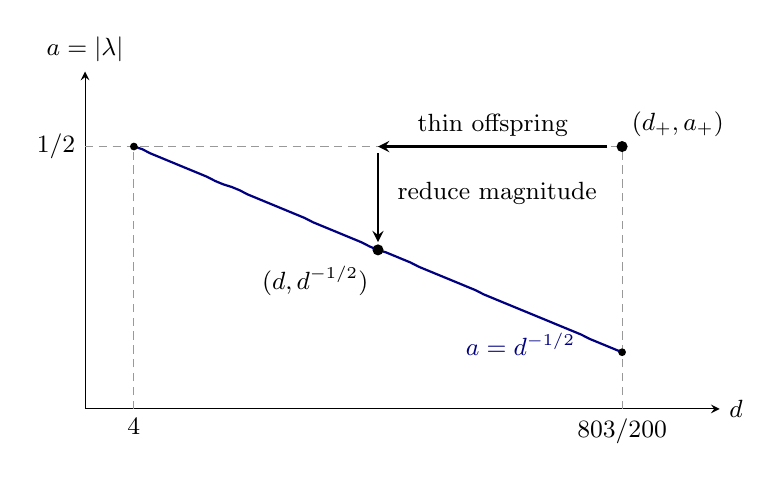
\begin{tikzpicture}[x=6.2cm,y=2.8cm,>=stealth,font=\small]
  \pgfmathsetmacro{\targety}{1000/sqrt(4+.015*.5)-499}
  \pgfmathsetmacro{\righty}{1000/sqrt(4+.015)-499}
  \draw[->] (-.10,-.19) -- (1.20,-.19) node[right] {$d$};
  \draw[->] (-.10,-.19) -- (-.10,1.34) node[above] {$a=|\lambda|$};
  \draw[densely dashed,black!40] (0,-.19) -- (0,1);
  \draw[densely dashed,black!40] (1,-.19) -- (1,1);
  \draw[densely dashed,black!40] (-.10,1) -- (1,1);
  \node[below] at (0,-.19) {$4$};
  \node[below] at (1,-.19) {$803/200$};
  \node[left] at (-.10,1) {$1/2$};
  \draw[thick,blue!50!black,domain=0:1,samples=61]
    plot (\x,{1000/sqrt(4+.015*\x)-499});
  \fill (0,1) circle (1.4pt);
  \fill (1,\righty) circle (1.4pt);
  \fill (1,1) circle (2pt);
  \node[above right] at (1,1) {$(d_+,a_+)$};
  \draw[->,thick] (.97,1) -- (.5,1)
    node[midway,above] {thin offspring};
  \draw[->,thick] (.5,.97) -- (.5,{\targety+.035});
  \node[right] at (.52,.79) {reduce magnitude};
  \fill (.5,\targety) circle (2pt);
  \node[below left] at (.5,{\targety-.03}) {$(d,d^{-1/2})$};
  \node[below right,text=blue!50!black] at (.66,.20)
    {$a=d^{-1/2}$};
\end{tikzpicture}
\caption{Domination in the first closed Poisson bin
$[4,803/200]$; the two axes use different enlarged scales.
The upper corner has $a_+=1/2$ and $d_+=803/200$, so it dominates
every equality experiment in the bin by thinning offspring and reducing
the channel magnitude.  It lies above the equality curve.
The certificate only brings its finite-depth upper law below $\mu=1/20$;
the local fixed-point gap is applied to the target equality experiment.}
\label{fig:dominating-bin}
\end{figure}

For each grid representative,
\[
 \left|\sum_i\frac{h_i}{H}\omega^i\right|^2
   =1-\frac{3(h_0h_1+h_1h_2+h_2h_0)}{H^2}.
\]
Define the integer
\begin{equation}
 M(m)=\sum_hm_h\bigl[H^2-3(h_0h_1+h_1h_2+h_2h_0)\bigr].
 \label{grid:moment}
\end{equation}
The certificate stops exactly when $20M(m)<NH^2$, equivalently
$\mu(m)<1/20$.  The exact code is included in
Section~\ref{cert:grid}.  With assertions enabled it returns iteration
$162$ for argument $-1$, the regular coloring recursion with four children at each vertex.
For arguments $j=0,\ldots,26$, the Poisson recursions return, in order,
\begin{equation}
\begin{gathered}
104,103,103,103,102,102,102,102,102,\\
101,101,101,101,101,101,\\
100,100,100,100,100,100,100,\\
99,99,99,99,99.
\end{gathered}
\label{grid:outputs}
\end{equation}
All comparisons determining these integers use exact integer arithmetic.
Appendix~\ref{grid:implementation} gives the bounds preventing overflow
and the correspondence between each code operation and the constructions
proved above.

\begin{proposition}[Completion of the negative threshold]
\label{grid:negative-completion}
For both tree models, every admissible negative parameter with
$da^2\leq1$ is non-reconstructible (with $d=b$ for a regular tree).
\end{proposition}
\begin{proof}
Consider first negative equality.  For the regular tree with $b=4$,
the upper law at depth $162$ has $\mu<1/20$.  For every Poisson
equality $d\in[4,881/200]$, choose a bin containing $d$ and its stopping
depth from~\eqref{grid:outputs}.  The corresponding upper law dominates
the exact equality depth experiment by the recursion and the two
garblings above.  Conditional Jensen gives
\mbox{$\mu_{\mathrm{true}}\leq\mu_{\mathrm{upper}}<1/20$} at that depth.
By Proposition~\ref{fnd:limit}, the actual depth laws have a symmetric
fixed-point limit and their moments decrease to its moment.  The limit
therefore has $\mu<1/20$ and is uniform by Proposition~\ref{loc:gap}.
This proves non-reconstruction in the certified range.

Proposition~\ref{fnd:limit} includes the coloring endpoint: its proof
extends the tilted recursion continuously across zero likelihood
normalizers and controls the Poisson count tail. Thus the preceding
fixed-point inference also applies at $a=1/2$.

Every remaining admissible regular equality has integer $b\geq5$ and
$a\leq1/\sqrt5<448/1000$.  Every remaining Poisson equality beyond
$881/200$ has $a<477/1000$ by~\eqref{grid:overlap}.
Proposition~\ref{wei:exclusion} excludes nonuniform fixed points in
these ranges, completing all negative equalities.

For $d\geq4$, every parameter $-d^{-1/2}\le\lambda<0$ is obtained by
the independent increment garbling from the equality parameter
$-1/\sqrt d$; hence its advantage also tends to zero.  For the remaining
parameters, first compare the coloring experiment with branching
parameter four to a smaller-branching coloring experiment.  For a
regular tree keep a fixed $b$ children at each vertex, and for a Poisson
tree retain each child with probability $d/4$, using the tree observation
and independent randomness.  This gives the smaller-tree observation
without the root.  Finally apply the increment garbling from $-1/2$ to
the desired negative parameter.  Thus all admissible negative channels
with branching parameter below four are non-reconstructible as well.
These are statements about the unconditional Poisson experiments, so
the conclusion uses exactly the averaging convention of the problem.
\end{proof}
